\chapter{Epidemic Models: How Diseases Spread}

\textit{This chapter builds the complete mathematical toolkit for modelling epidemic spreading from the ground up. We begin with a motivating story, introduce the SIR model's three compartments and two parameters, derive the governing differential equations term by term, simulate the model by hand using Euler's method, then progressively lift the model onto static networks, temporal networks, and finally into the stochastic Monte Carlo framework used by the project's \texttt{tsir/} simulation engine. Every symbol is defined before it is used. Every equation is computed with concrete numbers.}

% ============================================================
\section{Why We Need Models: A Motivating Story}
\label{sec:epi_motivation}
% ============================================================

\begin{analogybox}{The Epidemiologist's Question, March 2020}
Imagine you are a public-health official. The hospital data shows that 1\,000 people in your city are infected with a new respiratory virus today. Your director asks three questions:

\begin{enumerate}[noitemsep]
    \item \textbf{How many will be infected next week?}
    \item \textbf{Will the epidemic grow or burn out on its own?}
    \item \textbf{Who started it --- who was Patient Zero?}
\end{enumerate}

To answer any of these questions, you need a \emph{model}: a set of mathematical rules that describe how the disease moves from one person to another and at what rate people recover. Without a model, ``next week'' is a guess. With a model, it becomes a calculation.
\end{analogybox}

An \textbf{epidemic model} is a simplified, mathematical description of how a disease spreads through a population. The word ``simplified'' is important: no model captures every detail of biology, human behaviour, or geography. A good model captures the \emph{essential} mechanisms while remaining tractable enough to analyse.

Throughout this chapter, we build models of increasing realism:

\begin{enumerate}[noitemsep]
    \item \textbf{Well-mixed SIR} --- everyone meets everyone (a useful approximation).
    \item \textbf{Network SIR} --- contacts follow a graph; only neighbours can infect each other.
    \item \textbf{Temporal SIR} --- contacts are timestamped; the \emph{order} of meetings matters.
    \item \textbf{Stochastic simulation} --- the process is random; we run many realisations.
\end{enumerate}

Each step introduces new realism and new mathematical structure. The final model in this chapter is precisely the one implemented in the project's \texttt{tsir/} codebase.

\begin{keyinsight}{The Payoff: Why Models Enable Source Detection}
Once we have a model, we can \emph{run it in reverse}. Given an observed outbreak pattern (who is infected at time $T$), we can ask: ``which starting node would most plausibly produce this pattern?'' That is the source detection problem, formalised at the end of this chapter. The model is the bridge between ``what we see'' (the data) and ``what we want to know'' (who started it).
\end{keyinsight}

% ============================================================
\section{The SIR Model from First Principles}
\label{sec:sir_model}
% ============================================================

\subsection{Three States: What Each Person Can Be}

The SIR model divides every person in the population into exactly one of three \textbf{compartments} (states) at any given time:

\begin{conceptbox}{The Three SIR Compartments}
\begin{itemize}[noitemsep]
    \item \textbf{S --- Susceptible.} A healthy person who has not yet been infected and \emph{can} catch the disease if they come into contact with an infectious person. Think of them as ``at risk.''
    \item \textbf{I --- Infectious (Infected).} A person who currently carries the disease and \emph{can transmit it} to susceptible contacts. They are sick and contagious.
    \item \textbf{R --- Recovered (Removed).} A person who has had the disease and is now immune. They can no longer be infected and cannot infect others. They are ``out of play.''
\end{itemize}

Every person is in exactly one state at any moment: $S + I + R = N$, where $N$ is the total (fixed) population size.
\end{conceptbox}

The notation uses capital letters because they represent \emph{counts}: $S(t)$ is the number of susceptible people at time $t$, $I(t)$ is the number of infectious people, and $R(t)$ is the number of recovered people.

\begin{examplebox}{Reading $S + I + R = N$ Aloud}
In a town of $N = 1000$ people, suppose at time $t = 5$ days we have:
\[
S(5) = 850, \quad I(5) = 120, \quad R(5) = 30
\]
Check: $850 + 120 + 30 = 1000 = N$ \checkmark.

In words: 850 people are still healthy and could catch the disease; 120 are currently sick and contagious; 30 have already recovered and are immune. The epidemic is still growing (there are many susceptibles remaining).
\end{examplebox}

\subsection{The State Machine: How People Move Between States}

People move between states in one direction only. Once recovered, a person cannot become susceptible again (this is the key assumption of SIR; relaxing it gives the SIS model). The flow is:

\begin{center}
\begin{tikzpicture}[
  comp/.style={draw, rectangle, rounded corners=6pt, minimum width=2.2cm,
               minimum height=1.2cm, font=\bfseries\Large, thick},
  arr/.style={-{Stealth[length=4mm]}, thick, line width=2pt},
  lbl/.style={font=\small\sffamily, above, midway}
]
  \node[comp, fill=blue!15]  (S) at (0,0)    {$S$};
  \node[comp, fill=red!15]   (I) at (5.5,0)  {$I$};
  \node[comp, fill=green!15] (R) at (11.0,0) {$R$};

  \draw[arr] (S) -- node[lbl]{transmission} node[below, font=\small\sffamily, midway]{rate $\beta$} (I);
  \draw[arr] (I) -- node[lbl]{recovery}     node[below, font=\small\sffamily, midway]{rate $\mu$}   (R);

  % state labels below
  \node[font=\footnotesize\itshape, blue!60!black,  below=0.5cm] at (S) {Susceptible};
  \node[font=\footnotesize\itshape, red!60!black,   below=0.5cm] at (I) {Infectious};
  \node[font=\footnotesize\itshape, green!50!black, below=0.5cm] at (R) {Recovered};
\end{tikzpicture}
\end{center}

\subsection{Two Parameters: $\beta$ and $\mu$}

The SIR model is controlled by exactly two numbers:

\begin{conceptbox}{The Two SIR Parameters}
\textbf{$\beta$ (beta) --- Transmission rate.}
The probability per unit time that an infectious person transmits the disease to one susceptible contact. Concretely: if $\beta = 0.3$ per day, then an infectious person infects each of their susceptible contacts with probability $30\%$ per day.

\medskip
\textbf{$\mu$ (mu) --- Recovery rate.}
The probability per unit time that an infectious person recovers. The mean time spent in the infectious state is $1/\mu$ days. If $\mu = 0.1$ per day, the average infectious period is $1/0.1 = 10$ days.

\medskip
\textbf{Units:} Both $\beta$ and $\mu$ have units of $\text{time}^{-1}$ (per day, per hour, etc.), so their ratio $\beta/\mu$ is dimensionless.
\end{conceptbox}

\begin{analogybox}{$\beta$ and $\mu$ as Tap and Drain}
Think of the infectious compartment $I$ as a bucket of water.
\begin{itemize}[noitemsep]
    \item $\beta$ controls the \textbf{tap}: higher $\beta$ means more water flows in (more new infections per day).
    \item $\mu$ controls the \textbf{drain}: higher $\mu$ means water drains faster (people recover sooner).
\end{itemize}
If the tap flows faster than the drain, the bucket fills up (epidemic grows). If the drain wins, the bucket empties (epidemic dies out). The tipping point is exactly $\beta / \mu = 1$, which we will derive shortly.
\end{analogybox}

\subsection{The Differential Equations: Rate of Change of Each Compartment}

We now write down the mathematical rules governing how $S$, $I$, and $R$ change over time. We use \textbf{ordinary differential equations (ODEs)}: $dS/dt$ means ``the rate of change of $S$ with respect to time.'' A positive $dS/dt$ means $S$ is growing; a negative value means $S$ is shrinking.

We derive each equation in words first, then in symbols.

\subsubsection*{Rate of Change of $S$}

Susceptible people leave the $S$ compartment only when they get infected. The rate of new infections per unit time is proportional to:
\begin{itemize}[noitemsep]
    \item The number of infectious people $I(t)$ --- more sick people means more chances of contact.
    \item The number of susceptible people $S(t)$ --- more susceptibles means more people who can be infected.
    \item The transmission rate $\beta$ --- how easily the disease passes per contact.
    \item Divided by $N$ to reflect that contacts are spread across the whole population (well-mixed assumption).
\end{itemize}

This gives the rate $\beta \cdot S(t) \cdot I(t) / N$ new infections per unit time. Since these people \emph{leave} $S$, the sign is negative:

\begin{equation}
\frac{dS}{dt} = -\frac{\beta\, S(t)\, I(t)}{N}
\label{eq:sir_ds}
\end{equation}

\textbf{Reading aloud:} ``The rate of decrease of susceptibles equals beta times S times I, divided by the total population N.''

\subsubsection*{Rate of Change of $I$}

The infectious compartment gains people from $S$ (new infections) and loses people to $R$ (recoveries). The recovery rate is $\mu I(t)$: each of the $I(t)$ currently infectious people recovers at rate $\mu$.

\begin{equation}
\frac{dI}{dt} = \frac{\beta\, S(t)\, I(t)}{N} - \mu\, I(t)
\label{eq:sir_di}
\end{equation}

\textbf{Reading aloud:} ``The rate of change of infectious people equals the inflow of new infections (same magnitude as the outflow from $S$, so opposite sign) minus the outflow of recoveries.''

\subsubsection*{Rate of Change of $R$}

The recovered compartment only gains people from recoveries:

\begin{equation}
\frac{dR}{dt} = \mu\, I(t)
\label{eq:sir_dr}
\end{equation}

\textbf{Consistency check:} Adding all three equations, the $\beta SI/N$ terms cancel:
\[
\frac{dS}{dt} + \frac{dI}{dt} + \frac{dR}{dt} = -\frac{\beta SI}{N} + \frac{\beta SI}{N} - \mu I + \mu I = 0
\]
This means $S + I + R = N$ is constant for all time, as it should be. \checkmark

\begin{mathbox}{The SIR ODE System (Complete)}
\begin{align}
    \frac{dS}{dt} &= -\frac{\beta\, S(t)\, I(t)}{N} \tag{\ref{eq:sir_ds}} \\[4pt]
    \frac{dI}{dt} &= \frac{\beta\, S(t)\, I(t)}{N} - \mu\, I(t) \tag{\ref{eq:sir_di}} \\[4pt]
    \frac{dR}{dt} &= \mu\, I(t) \tag{\ref{eq:sir_dr}}
\end{align}
\textbf{Parameters:} $\beta > 0$ (transmission rate), $\mu > 0$ (recovery rate), $N$ (fixed population).\\
\textbf{Initial conditions:} $S(0) = N - I_0 - R_0$, typically $I_0 = 1$ (one index case), $R_0 = 0$.\\
\textbf{Conservation:} $S(t) + I(t) + R(t) = N$ for all $t \geq 0$.
\end{mathbox}

\subsection{Numerical Simulation by Hand: Euler's Method}

The SIR system has no simple closed-form solution (unlike the SI model). We simulate it numerically using the simplest method: \textbf{Euler's method}. The idea is elementary: if we know the state at time $t$, and we know the \emph{rate of change} at that moment, we can approximate the state at time $t + \Delta t$ by stepping forward:

\[
X(t + \Delta t) \approx X(t) + \frac{dX}{dt}\bigg|_t \cdot \Delta t
\]

``The new value equals the old value plus the rate of change times the time step.''

\begin{examplebox}{Euler's Method Applied to SIR: Step-by-Step Computation}
\textbf{Setup:} $N = 100$, $S(0) = 99$, $I(0) = 1$, $R(0) = 0$, $\beta = 0.3$, $\mu = 0.1$, $\Delta t = 1$ day.

\medskip
\textbf{Step 1: Compute rates at $t = 0$.}
\begin{align*}
    \frac{dS}{dt}\bigg|_0 &= -\frac{0.3 \times 99 \times 1}{100} = -\frac{29.7}{100} = -0.297 \\[4pt]
    \frac{dI}{dt}\bigg|_0 &= +0.297 - 0.1 \times 1 = 0.297 - 0.100 = +0.197 \\[4pt]
    \frac{dR}{dt}\bigg|_0 &= 0.1 \times 1 = +0.100
\end{align*}

\medskip
\textbf{Step 2: Advance to $t = 1$ day.}
\begin{align*}
    S(1) &= S(0) + \frac{dS}{dt}\big|_0 \cdot \Delta t = 99 + (-0.297)(1) = 98.703 \\
    I(1) &= I(0) + \frac{dI}{dt}\big|_0 \cdot \Delta t = 1 + (+0.197)(1) = 1.197 \\
    R(1) &= R(0) + \frac{dR}{dt}\big|_0 \cdot \Delta t = 0 + (+0.100)(1) = 0.100
\end{align*}

\textbf{Check:} $98.703 + 1.197 + 0.100 = 100.000 = N$ \checkmark

\medskip
\textbf{Step 3: Repeat with updated values at $t = 1$.}
\begin{align*}
    \frac{dS}{dt}\bigg|_1 &= -\frac{0.3 \times 98.703 \times 1.197}{100} = -\frac{35.448}{100} = -0.354 \\[4pt]
    \frac{dI}{dt}\bigg|_1 &= +0.354 - 0.1 \times 1.197 = 0.354 - 0.120 = +0.234 \\[4pt]
    \frac{dR}{dt}\bigg|_1 &= 0.1 \times 1.197 = +0.120
\end{align*}
\begin{align*}
    S(2) &= 98.703 - 0.354 = 98.349 \\
    I(2) &= 1.197 + 0.234 = 1.431 \\
    R(2) &= 0.100 + 0.120 = 0.220
\end{align*}

\medskip
\textbf{Three-step summary:}
\begin{center}
\begin{tabular}{ccccc}
\toprule
$t$ & $S(t)$ & $I(t)$ & $R(t)$ & $S+I+R$ \\
\midrule
0 & 99.000 & 1.000 & 0.000 & 100.000 \\
1 & 98.703 & 1.197 & 0.100 & 100.000 \\
2 & 98.349 & 1.431 & 0.220 & 100.000 \\
\bottomrule
\end{tabular}
\end{center}

\textbf{Interpretation:} In the first two days, $I$ is growing (epidemic expanding) while $S$ slowly depletes. The epidemic has not yet peaked.

\medskip
\textbf{Why does $I$ grow?} Because $dI/dt = \beta SI/N - \mu I > 0$ when $\beta S/N > \mu$, i.e., when $S > \mu N/\beta = 0.1 \times 100/0.3 \approx 33$. As long as more than 33 people remain susceptible, the epidemic grows.
\end{examplebox}

\subsection{The Basic Reproduction Number $R_0$}

The single most important quantity in epidemiology is the \textbf{basic reproduction number}, written $R_0$ (pronounced ``R-naught'').

\begin{conceptbox}{The Basic Reproduction Number $R_0$}
$R_0$ is the average number of secondary infections caused by a single infectious individual introduced into a \emph{fully susceptible} population.

In the well-mixed SIR model:
\begin{equation}
    R_0 = \frac{\beta}{\mu}
    \label{eq:r0}
\end{equation}
\textbf{Reading aloud:} ``R-naught equals the transmission rate divided by the recovery rate.''

\textbf{Why this formula?} An infectious person infects at rate $\beta$ per susceptible contact. In a fully susceptible population of size $N$, each person has $\approx N$ potential contacts. The mean infectious duration is $1/\mu$ days. So the total number of secondary infections is $\beta \cdot (1/\mu) = \beta/\mu$.

\textbf{The threshold:}
\begin{itemize}[noitemsep]
    \item If $R_0 > 1$: Each case produces more than one new case on average. The epidemic grows.
    \item If $R_0 = 1$: Exactly self-sustaining. The epidemic neither grows nor shrinks.
    \item If $R_0 < 1$: Each case produces fewer than one new case on average. The epidemic dies out.
\end{itemize}
\end{conceptbox}

\begin{examplebox}{Computing $R_0$ for $\beta = 0.3$, $\mu = 0.1$}
\[
R_0 = \frac{\beta}{\mu} = \frac{0.3}{0.1} = 3
\]
\textbf{Interpretation:} On average, one infected person infects \emph{3 others} (in a fully susceptible population). This is approximately the $R_0$ of seasonal influenza. The epidemic will spread.

For our Euler simulation above ($S(0) = 99 \approx N$, close to fully susceptible): since $R_0 = 3 > 1$, the epidemic grows, as we observed in the computation.

\textbf{To stop the epidemic:} We need to reduce $R_0$ below 1. One way is vaccination: if a fraction $1 - 1/R_0 = 1 - 1/3 \approx 67\%$ of the population is immune, the effective $R_0$ drops below 1. This is the \textbf{herd immunity threshold}.
\end{examplebox}

\begin{center}
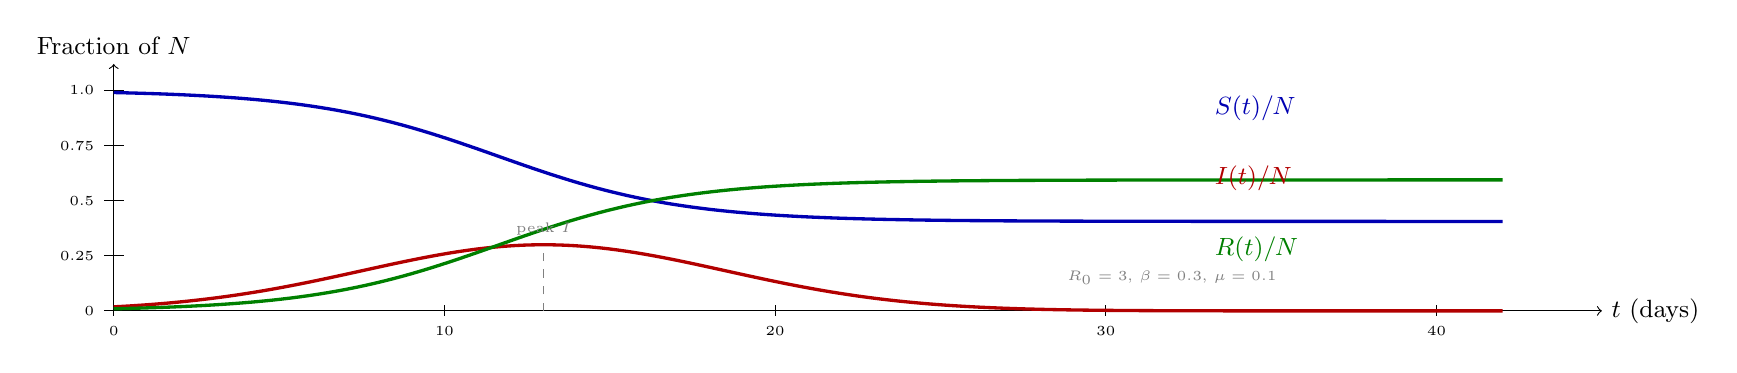
\begin{tikzpicture}[scale=1.0]
\begin{scope}[xscale=0.42, yscale=2.8]
  % Axes
  \draw[->] (0,0) -- (45,0) node[right]{\small $t$ (days)};
  \draw[->] (0,0) -- (0,1.12) node[above]{\small Fraction of $N$};
  \foreach \x in {0,10,20,30,40}{
    \draw (\x,0.025) -- (\x,-0.025) node[below]{\tiny\x};
  }
  \foreach \y in {0,0.25,0.5,0.75,1.0}{
    \draw (0.3,\y) -- (-0.3,\y) node[left]{\tiny\y};
  }
  % Approximate SIR curves: beta=0.3, mu=0.1, R0=3, N=100, S0=99, I0=1
  % S(t): starts near 1, declines to ~0.06 (final size ~94%)
  \draw[blue!70!black, very thick, domain=0:42, samples=150]
    plot (\x, {0.06 + 0.94 * exp(-1.0/(1+exp(-0.35*(\x-13))))});
  % I(t): bell, peaks ~t=13 at ~0.28
  \draw[red!70!black, very thick, domain=0:42, samples=150]
    plot (\x, {0.30*exp(-0.5*((\x-13)/5.5)^2)});
  % R(t): sigmoid from 0 to ~0.94
  \draw[green!50!black, very thick, domain=0:42, samples=150]
    plot (\x, {0.94*(1-exp(-1.0/(1+exp(-0.35*(\x-13)))))});
  % Peak marker
  \draw[gray, dashed] (13, 0) -- (13, 0.30);
  \node[font=\tiny, gray, above] at (13, 0.30) {peak $I$};
  % Legend
  \node[blue!70!black,  font=\small, right] at (33, 0.92) {$S(t)/N$};
  \node[red!70!black,   font=\small, right] at (33, 0.60) {$I(t)/N$};
  \node[green!50!black, font=\small, right] at (33, 0.28) {$R(t)/N$};
  % Annotation: epidemic peak
  \node[font=\tiny, gray] at (32, 0.15) {$R_0 = 3$, $\beta=0.3$, $\mu=0.1$};
\end{scope}
\end{tikzpicture}
\end{center}

\begin{keyinsight}{The Three Phases of an SIR Epidemic}
\begin{enumerate}[noitemsep]
    \item \textbf{Exponential growth} (early stage): $S \approx N$, so $dI/dt \approx \beta I - \mu I = (\beta - \mu) I$. The number of infected grows exponentially at rate $\beta - \mu$. This is why early intervention matters so much.
    \item \textbf{Peak and decline} (middle stage): $S$ has been depleted enough that $\beta S(t)/N < \mu$. New infections no longer outpace recoveries; $I$ peaks and then falls.
    \item \textbf{Burnout} (late stage): the epidemic ends not because everyone is vaccinated, but because there are not enough susceptibles left to sustain transmission. Some susceptibles always survive.
\end{enumerate}
\end{keyinsight}

% ============================================================
\section{The SIR Model on Networks (Network SIR)}
\label{sec:network_sir}
% ============================================================

\subsection{Why the Well-Mixed Assumption Fails}

The well-mixed SIR model assumes that every person can potentially infect every other person. In reality, you can only infect someone you actually meet. Your contacts follow a \textbf{network structure}: your family, colleagues, neighbours, and friends. A hermit with no contacts cannot infect anyone, regardless of how infectious they are. A highly connected person (a doctor, a teacher, a flight attendant) can infect many.

\begin{analogybox}{The Network Changes Everything}
Imagine two towns. Town A is a bus network: everyone goes through the central hub station. Town B is a grid of streets: everyone moves locally. Introduce an infected traveller into the hub of Town A --- the disease reaches all corners of town within days. Introduce the same traveller into a corner of Town B --- the disease spreads slowly, touching each block one by one. Same $\beta$, same $\mu$, same $R_0$. But the dynamics are completely different because the contact \emph{structure} is different.
\end{analogybox}

\subsection{Network SIR: One State per Node}

In the network-aware SIR model, we assign a state $X_i(t) \in \{S, I, R\}$ to \emph{each individual node} $i$. Instead of population-level counts, we track individual fates.

The contact structure is a graph $G = (\mathcal{V}, \mathcal{E})$ where $\mathcal{V}$ is the set of $N$ people (nodes) and $\mathcal{E}$ is the set of contacts (edges). An edge $\{i,j\} \in \mathcal{E}$ means person $i$ and person $j$ are in contact and can transmit the disease to each other.

\subsection{Per-Node Infection Probability}

At each discrete time step, a susceptible node $v$ can be infected by each of its \emph{infectious neighbours} independently. The probability that \emph{at least one} infectious neighbour infects $v$ in one time step is:

\begin{mathbox}{Per-Node Infection Probability (Independent Contacts)}
Let $\mathcal{N}_I(v, t) = \{u \in \mathcal{N}(v) \mid X_u(t) = I\}$ be the set of infectious neighbours of $v$ at time $t$. Each infectious neighbour independently fails to infect $v$ with probability $(1 - \beta)$. All $|\mathcal{N}_I(v,t)|$ must fail for $v$ to remain susceptible. Therefore:

\begin{equation}
    P\bigl(v \text{ gets infected at } t\bigr) = 1 - \prod_{u \in \mathcal{N}_I(v,t)} (1 - \beta)
    = 1 - (1-\beta)^{|\mathcal{N}_I(v,t)|}
    \label{eq:network_infection}
\end{equation}

\textbf{Reading aloud:} ``The probability that $v$ gets infected equals one minus the product over all infectious neighbours of $(1 - \beta)$.''

\textbf{Why a product?} Each infection attempt by a different neighbour is \emph{independent}. The probability that ALL of them fail is the product of each failure probability. One minus that product is the probability that at least one succeeds.
\end{mathbox}

\begin{examplebox}{Computing Infection Probability: Node $v$ with 3 Infected Neighbours}
Node $v$ has 3 infectious neighbours (call them $u_1, u_2, u_3$) and $\beta = 0.2$.

\medskip
\textbf{Step 1:} Each infected neighbour fails to infect $v$ with probability $1 - \beta = 1 - 0.2 = 0.8$.

\medskip
\textbf{Step 2:} All three fail simultaneously with probability $0.8 \times 0.8 \times 0.8 = (0.8)^3 = 0.512$.

\medskip
\textbf{Step 3:} At least one succeeds (i.e., $v$ gets infected) with probability:
\[
P(\text{infected}) = 1 - (0.8)^3 = 1 - 0.512 = \mathbf{0.488}
\]

\textbf{Interpretation:} Even with a relatively low per-contact transmission rate ($\beta = 0.2$), having 3 infected neighbours gives nearly a 50\% chance of being infected in this time step.

\medskip
\textbf{Contrast with 1 infected neighbour:} $P = 1 - 0.8^1 = 0.2$ (exactly $\beta$, as expected).\\
\textbf{With 5 infected neighbours:} $P = 1 - 0.8^5 = 1 - 0.328 = 0.672$ (67\%!).

This shows why \textbf{hubs} (highly connected nodes) are so dangerous: when they are infected, they expose many neighbours simultaneously, driving high infection probabilities even for moderate $\beta$.
\end{examplebox}

\subsection{How the Network Changes Spreading Dynamics}

The network structure modifies both the speed and pattern of spread:

\begin{itemize}
    \item \textbf{Hub nodes} (high degree): a node with degree $k = 50$ can expose 50 people simultaneously. If it becomes infected, it creates a ``burst'' of new cases. In scale-free networks, these hubs collapse the diameter and cause the epidemic to spread much faster than the well-mixed model would predict.
    \item \textbf{Dead-end nodes} (low degree): a node with only 1 contact (a leaf node) can infect at most one person. Stochastic extinction is common from such nodes.
    \item \textbf{Community structure}: if the network consists of tightly-knit clusters connected by a few ``bridge'' edges, the epidemic spreads quickly within each cluster but may take a long time to jump between clusters.
\end{itemize}

\begin{keyinsight}{$R_0$ on a Heterogeneous Network}
In a network where the degree distribution has mean $\langle k \rangle$ and variance $\sigma_k^2$, the effective reproduction number is (via heterogeneous mean-field theory):
\begin{equation}
    R_0^{\mathrm{network}} = \frac{\beta}{\mu} \cdot \frac{\langle k^2 \rangle - \langle k \rangle}{\langle k \rangle}
    \label{eq:r0_network}
\end{equation}
The additional factor $(\langle k^2 \rangle - \langle k \rangle)/\langle k \rangle$ is the \textbf{mean excess degree}: the average number of additional neighbours reachable by following a random edge. For a Poisson degree distribution (Erd\H{o}s-R\'enyi networks), this equals $\langle k \rangle$, recovering $R_0^{\mathrm{network}} = \beta \langle k \rangle / \mu$. For scale-free networks where variance $\sigma_k^2 \gg \langle k \rangle^2$, $R_0^{\mathrm{network}}$ is enormous, explaining why these networks are nearly impossible to make epidemic-free by random vaccination.
\end{keyinsight}

% ============================================================
\section{Temporal SIR on Temporal Networks}
\label{sec:temporal_sir}
% ============================================================

\subsection{Why the Order of Contacts Matters}

In a static network, the edge $\{i, j\}$ says ``$i$ and $j$ are in contact.'' It does not say \emph{when}. This is a problem because diseases cannot travel backwards in time.

\begin{examplebox}{Temporal Order Changes Everything: A 3-Node Example}
Consider three people: Alice (A), Bob (B), and Charlie (C). Suppose the following contacts occur:
\begin{itemize}[noitemsep]
    \item Contact event $e_1$: A meets B at time $t = 1$.
    \item Contact event $e_2$: B meets C at time $t = 2$.
\end{itemize}

\textbf{Scenario 1 (A is the source, infects at $t=1$):}
\begin{itemize}[noitemsep]
    \item At $t=1$: A meets B. A is infected, so B can be infected ($\beta$ transmission attempt). \textbf{Possible path: A $\to$ B $\to$ C.}
    \item At $t=2$: B (if infected) meets C. \textbf{C can be infected by B.}
\end{itemize}

\textbf{Now reverse the order of events:} Suppose instead:
\begin{itemize}[noitemsep]
    \item Contact event $e_1'$: B meets C at time $t = 1$.
    \item Contact event $e_2'$: A meets B at time $t = 2$.
\end{itemize}

\textbf{Scenario 2 (same contacts, different order, A is the source):}
\begin{itemize}[noitemsep]
    \item At $t=1$: B meets C. A is still the only infected person. B is susceptible, so \textbf{nothing happens} (no transmission source for C from B yet).
    \item At $t=2$: A meets B. Now B can be infected. But the B--C contact already happened at $t=1$ when B was susceptible. \textbf{C cannot be infected via B.}
\end{itemize}

\textbf{Result:} Same contact graph (A--B--C path), same parameters, same source (A). But Scenario 1 allows C to be infected, while Scenario 2 does not. The temporal order of contacts is the difference.
\end{examplebox}

\begin{center}
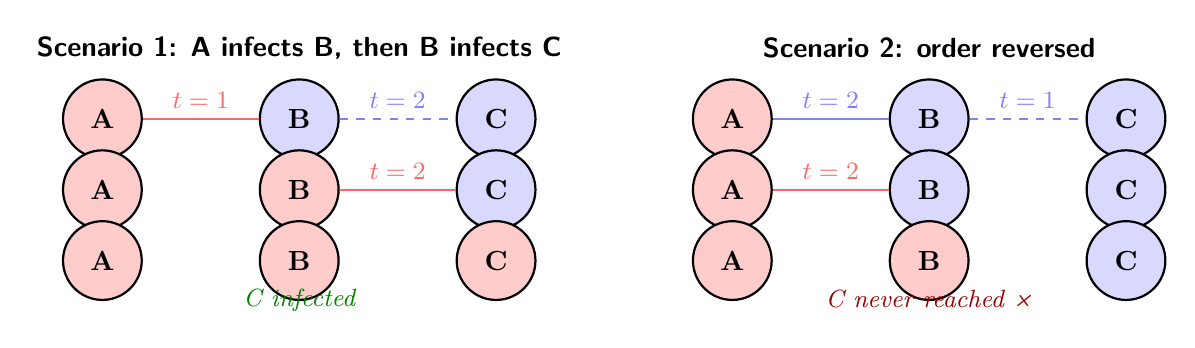
\begin{tikzpicture}[
  pnode/.style={draw, circle, minimum size=1.0cm, font=\bfseries, thick},
  Sn/.style={pnode, fill=blue!15},
  In/.style={pnode, fill=red!20},
  arr/.style={-{Stealth[length=3mm]}, thick}
]
% Scenario 1
\node[font=\bfseries\sffamily] at (2.5, 3.3) {Scenario 1: A infects B, then B infects C};

\node[In]  (A1) at (0.0, 2.4) {A};
\node[Sn]  (B1) at (2.5, 2.4) {B};
\node[Sn]  (C1) at (5.0, 2.4) {C};
\draw[thick, red!60] (A1) -- node[above, font=\small]{$t=1$} (B1);
\draw[thick, blue!50, dashed] (B1) -- node[above, font=\small]{$t=2$} (C1);

\node[In]  (A1b) at (0.0, 1.5) {A};
\node[In]  (B1b) at (2.5, 1.5) {B};
\node[Sn]  (C1b) at (5.0, 1.5) {C};
\draw[thick, red!60] (B1b) -- node[above, font=\small]{$t=2$} (C1b);

\node[In]  (A1c) at (0.0, 0.6) {A};
\node[In]  (B1c) at (2.5, 0.6) {B};
\node[In]  (C1c) at (5.0, 0.6) {C};
\node[font=\small\itshape, green!50!black] at (2.5, 0.1) {C infected \checkmark};

% Scenario 2
\node[font=\bfseries\sffamily] at (10.5, 3.3) {Scenario 2: order reversed};

\node[In]  (A2) at (8.0, 2.4) {A};
\node[Sn]  (B2) at (10.5, 2.4) {B};
\node[Sn]  (C2) at (13.0, 2.4) {C};
\draw[thick, blue!50, dashed] (B2) -- node[above, font=\small]{$t=1$} (C2);
\draw[thick, blue!50] (A2) -- node[above, font=\small]{$t=2$} (B2);

\node[In]  (A2b) at (8.0, 1.5) {A};
\node[Sn]  (B2b) at (10.5, 1.5) {B};
\node[Sn]  (C2b) at (13.0, 1.5) {C};
\draw[thick, red!60] (A2b) -- node[above, font=\small]{$t=2$} (B2b);

\node[In]  (A2c) at (8.0, 0.6) {A};
\node[In]  (B2c) at (10.5, 0.6) {B};
\node[Sn]  (C2c) at (13.0, 0.6) {C};
\node[font=\small\itshape, red!60!black] at (10.5, 0.1) {C never reached \texttimes};

\end{tikzpicture}

\vspace{0.5em}
\small\itshape
Red solid edges: active transmission. Blue dashed edges: contact with no transmission (one side not yet infected). Same network topology, same parameters --- different temporal order gives a different outcome.
\end{center}

\subsection{Temporal Networks as Event Sequences}

A \textbf{temporal network} $G^T = (\mathcal{V}, E^T)$ is a list of timestamped contact events:
\[
E^T = \{(u_1, v_1, t_1),\; (u_2, v_2, t_2),\; \ldots,\; (u_m, v_m, t_m)\}
\]
where each triple $(u, v, t)$ means ``person $u$ and person $v$ were in contact at time $t$.'' The events are sorted by time: $t_1 \leq t_2 \leq \cdots \leq t_m$.

\subsection{Discrete-Time Temporal SIR: The Simulation Rule}

The simulation processes events in chronological order. At each contact event $(u, v, t)$:

\begin{conceptbox}{The Temporal SIR Update Rule}
When a contact event $(u, v, t)$ is processed:
\begin{enumerate}[noitemsep]
    \item \textbf{Attempt infection} from $u$ to $v$: if $X_u(t) = I$ and $X_v(t) = S$, then $v$ becomes infected with probability $\beta$. (Draw a uniform random number; if it is $< \beta$, set $X_v \leftarrow I$.)
    \item \textbf{Attempt infection} from $v$ to $u$: symmetrically, if $X_v(t) = I$ and $X_u(t) = S$, then $u$ becomes infected with probability $\beta$.
    \item \textbf{Recovery}: between events, each infectious node $i$ recovers with probability $\mu$ per unit time. In an event-driven simulation, this is handled by sampling the recovery time for each node when they become infected.
\end{enumerate}
\end{conceptbox}

\begin{conceptbox}{The Infectious Window}
A node can only spread the infection while it is in state $I$. Once a node recovers (transitions to $R$), any subsequent contact events involving that node are irrelevant for transmission. This is the \textbf{infectious window}: the time interval between a node's infection time and recovery time.

If node $i$ is infected at time $t_{\text{inf}}$ and recovers at time $t_{\text{rec}} \sim \text{Exponential}(\mu)$, then node $i$ can only infect neighbours during the interval $[t_{\text{inf}}, t_{\text{rec}})$. Contact events $(i, j, t)$ with $t \geq t_{\text{rec}}$ are ignored.

This creates an \textbf{asymmetry}: if $i$ infects $j$ early in its infectious window, $j$ has the rest of the observation period to potentially spread further. If $i$ infects $j$ late, $j$ has little time. The temporal structure of the contact sequence directly shapes the final outbreak pattern.
\end{conceptbox}

\begin{examplebox}{Three Nodes, Two Events: Computing Temporal SIR by Hand}
\textbf{Network:} 3 nodes $\{A, B, C\}$. Events: $(A, B, t=2)$ and $(B, C, t=5)$.

\textbf{Parameters:} $\beta = 0.6$. Recovery times are drawn from Exponential($\mu=0.1$), so mean infectious period $= 10$ time units.

\textbf{Initial state:} $A$ is infected at $t=0$ (source). $B$ and $C$ are susceptible.

\textbf{Draw recovery time for A:} Suppose $t_{\text{rec}}(A) = 8$ (a random sample).

\medskip
\textbf{Process event $(A, B, t=2)$:}
\begin{itemize}[noitemsep]
    \item $t = 2 < t_{\text{rec}}(A) = 8$ --- A is still infectious. \checkmark
    \item $X_B(2) = S$ --- B is susceptible. \checkmark
    \item Draw $U \sim \text{Uniform}(0,1)$. Suppose $U = 0.41 < \beta = 0.6$. \textbf{B gets infected.}
    \item Draw $t_{\text{rec}}(B) \sim \text{Exponential}(0.1)$. Suppose $t_{\text{rec}}(B) = 13$.
\end{itemize}

\textbf{Process event $(B, C, t=5)$:}
\begin{itemize}[noitemsep]
    \item $t = 5 < t_{\text{rec}}(B) = 13$ --- B is still infectious. \checkmark
    \item $X_C(5) = S$ --- C is susceptible. \checkmark
    \item Draw $U = 0.75 > \beta = 0.6$. \textbf{C is not infected.} (Lucky escape.)
\end{itemize}

\textbf{Final state (after all recoveries):} $A \in R$, $B \in R$, $C \in S$. Only $A$ and $B$ were infected.

\textbf{If instead $t_{\text{rec}}(A) = 1$ (recovers before $t=2$):} Then event $(A, B, t=2)$ does nothing (A already in $R$), and the entire epidemic dies with only A infected. The randomness of recovery timing creates dramatically different outcomes from the same source.
\end{examplebox}

% ============================================================
\section{Stochastic Simulations (Monte Carlo)}
\label{sec:monte_carlo}
% ============================================================

\subsection{Why One Run Is Not Enough}

The temporal SIR process is \textbf{stochastic} (random). Given a fixed source node $v_0$ and fixed parameters $\beta$ and $\mu$, running the simulation twice will generally produce two different final states. Sometimes the epidemic explodes and infects 80\% of the network; sometimes it dies out after 3 nodes. Both outcomes can arise from the same source.

\begin{analogybox}{Stochastic Epidemics as Dice Rolls}
Imagine rolling a die at each contact event: if you roll a 1 or 2 (on a six-sided die, i.e., $\beta = 1/3$), the infection passes. Each ``run'' is a different sequence of dice rolls. Run the experiment 1000 times and you see the full distribution of outcomes: sometimes all dice roll high (big outbreak), sometimes all roll low (early extinction). The probability distribution over outcomes characterises the source's epidemiological ``fingerprint.''
\end{analogybox}

This randomness means that to characterise how a source behaves, we must run \textbf{many} simulations and look at the distribution. This is \textbf{Monte Carlo simulation}: using random sampling to estimate probability distributions.

\subsection{Terminology: $n\_\text{runs}$ and $\text{mc\_runs}$}

The project codebase distinguishes two roles for simulations:

\begin{conceptbox}{Two Types of Simulation Runs}
\textbf{\texttt{n\_runs}} (ground-truth runs): For each candidate source node $v_0 \in \mathcal{V}$, we run \texttt{n\_runs} independent SIR simulations from $v_0$. These high-statistics runs are used to compute the \emph{ground-truth likelihood} $P(\mathcal{O} \mid \text{source} = v_0)$. Default: \texttt{n\_runs} = 5000.

\medskip
\textbf{\texttt{mc\_runs}} (Monte Carlo training runs): Additional simulations run from each node, used to generate \emph{training data} for the GNN. These are observations the model learns from. Default: \texttt{mc\_runs} = 500.

\medskip
\textbf{Why different sizes?} The ground-truth likelihood needs high precision (5000 runs $\to$ standard error $\leq 0.007$) because it is the reference we compare against. Training data can tolerate more noise (500 runs) to keep data generation tractable.
\end{conceptbox}

\subsection{Pseudocode for a Single Temporal SIR Simulation}

\begin{codewalk}{Single Temporal SIR Simulation: Pseudocode}
\begin{lstlisting}[language=Python]
def run_temporal_sir(events, n_nodes, beta, mu, source):
    """
    Run one stochastic SIR simulation on a temporal network.

    Parameters
    ----------
    events   : list of (u, v, t) triples, sorted by ascending t
    n_nodes  : total number of nodes
    beta     : transmission probability per contact event
    mu       : recovery rate (per unit time)
    source   : index of the initial infectious node

    Returns
    -------
    state    : np.array of shape (n_nodes,), dtype int8
               0 = Susceptible, 1 = Infected, 2 = Recovered
               (state at the END of the simulation)
    """
    # --- Initialisation ---
    state = np.zeros(n_nodes, dtype=int8)      # all Susceptible
    state[source] = 1                           # source is Infected
    infection_time = {source: 0.0}             # when each node was infected
    recovery_time  = {}                         # when each node will recover

    # Draw recovery time for the source
    recovery_time[source] = 0.0 + sample_exponential(mu)

    # --- Process events in chronological order ---
    for (u, v, t) in sorted(events, key=lambda e: e[2]):

        # Attempt infection u -> v
        if state[u] == 1 and state[v] == 0:         # u infectious, v susceptible
            if t < recovery_time[u]:                 # u still in infectious window
                if random.uniform(0,1) < beta:       # transmission succeeds
                    state[v] = 1
                    infection_time[v] = t
                    recovery_time[v] = t + sample_exponential(mu)

        # Attempt infection v -> u (symmetric)
        if state[v] == 1 and state[u] == 0:
            if t < recovery_time[v]:
                if random.uniform(0,1) < beta:
                    state[u] = 1
                    infection_time[u] = t
                    recovery_time[u] = t + sample_exponential(mu)

    # --- Mark all infectious nodes as Recovered at end ---
    for i in range(n_nodes):
        if state[i] == 1:
            state[i] = 2

    return state
\end{lstlisting}
\textbf{Key points:}
\begin{itemize}[noitemsep]
    \item Events are processed in time order (line 23). This enforces the causal ordering.
    \item The \texttt{recovery\_time[u]} check (line 26) implements the infectious window.
    \item \texttt{sample\_exponential(mu)} returns a sample from the exponential distribution with mean $1/\mu$.
    \item The output is a flat array of shape \texttt{(n\_nodes,)} with values in $\{0, 1, 2\}$ for $\{S, I, R\}$.
\end{itemize}
\end{codewalk}

\subsection{The Output: Binary Arrays and Their Shape}

Running \texttt{n\_runs} simulations from a single source node $v_0$ produces \texttt{n\_runs} state vectors, each of shape \texttt{(n\_nodes,)}. Stacking them gives an array of shape \texttt{(n\_runs, n\_nodes)}.

When we run \texttt{n\_runs} simulations from \emph{every} possible source node, we get an array of shape \texttt{(n\_nodes, n\_runs, n\_nodes)}.

\begin{conceptbox}{The \texttt{truth\_S/I/R} Array Shape: \texttt{(n\_nodes, n\_runs, n\_nodes)}}
The three arrays \texttt{truth\_S}, \texttt{truth\_I}, \texttt{truth\_R} each have shape \texttt{(n\_nodes, n\_runs, n\_nodes)} and contain values in $\{0, 1\}$ (int8).

\textbf{Axis 0 --- source node index:} Which node was used as the source for this batch of simulations. \texttt{truth\_I[v, :, :]} contains all simulation runs with source $v$.

\textbf{Axis 1 --- simulation run index:} The run number within the batch. \texttt{truth\_I[v, r, :]} is the state vector from the $r$-th run with source $v$.

\textbf{Axis 2 --- node state:} Whether each node is in state $I$ (or $S$, or $R$) at the end. \texttt{truth\_I[v, r, j] = 1} means node $j$ was infectious at the end of run $r$ with source $v$.

\textbf{Example access:}
\begin{lstlisting}[language=Python]
# Fraction of runs from source v=3 in which node j=7 was infected:
fraction_infected = truth_I[3, :, 7].mean()   # mean over all n_runs

# All final states from source v=0, run r=42:
state_vector = truth_I[0, 42, :]   # shape (n_nodes,)
\end{lstlisting}

\medskip
\textbf{Memory:} For $N = 500$ nodes, $n\_\text{runs} = 5000$: each array is $500 \times 5000 \times 500 = 1.25 \times 10^9$ entries. At 1 byte (int8) each, that is approximately 1.25 GB per array (times 3 for S, I, R). This is why the simulation data is stored in compact binary \texttt{.bin} files and loaded via \texttt{np.fromfile}.
\end{conceptbox}

Similarly, the Monte Carlo training arrays \texttt{mc\_S/I/R} have shape \texttt{(n\_nodes, mc\_runs, n\_nodes)}, where \texttt{mc\_runs} $\ll$ \texttt{n\_runs}.

% ============================================================
\section{The TSIR C Implementation}
\label{sec:tsir_code}
% ============================================================

\subsection{Why C for Simulation?}

Running $N \times n\_\text{runs}$ simulations in Python would take hours. The project uses an event-driven C implementation of temporal SIR adapted from Petter Holme's \texttt{tsir} codebase (see \cite{holme2020fast}), wrapped in a Python interface. The C code processes all events for all nodes in a tight loop with no Python interpreter overhead, achieving speedups of 100--1000$\times$ over equivalent Python code.

\subsection{The Python Wrapper: How to Call the Simulation}

\begin{codewalk}{Calling the TSIR C Engine from Python (\texttt{tsir/read\_run.py})}
The Python layer provides three functions, each running the C binary with different parameters:

\begin{lstlisting}[language=Python]
from tsir.read_run import tsir, make_c_readable_from_nparray

# Step 1: Convert the temporal network to the C-readable text format.
# H_array is a NumPy array of shape (n_events, 3) with columns [u, v, t].
H_cedges = make_c_readable_from_nparray(H_array, end_t, n_nodes)

# Step 2: Configure the simulation.
tsir_config = {
    "sir": {
        "beta":    0.3,    # transmission rate
        "mu":      0.1,    # recovery rate
        "start_t": 0,      # first event time to include
        "end_t":   50,     # last event time (observation cutoff)
        "n_runs":  5000    # number of simulations per source
    },
    "nwk": {
        "directed": False  # undirected contact network
    }
}

# Step 3: Run the simulation.
# Returns three arrays: log-probabilities of S, I, R per node.
tsir_S, tsir_I, tsir_R = tsir(tsir_config, H_cedges, n_nodes)
\end{lstlisting}

Internally, \texttt{tsir()} calls the compiled C binary \texttt{./tsir/tsir} via subprocess, passing the network as a pipe, and reads back three binary \texttt{.bin} files containing the output arrays.
\end{codewalk}

\subsection{The Ground-Truth and Monte Carlo Functions}

The \texttt{read\_run.py} module exposes two higher-level functions that wrap the C binary for the two use cases:

\begin{codewalk}{Ground-Truth and Monte Carlo Runs (\texttt{tsir/read\_run.py})}
\begin{lstlisting}[language=Python]
# --- Ground-truth run (high n_runs, one per source node) ---
truth_S, truth_I, truth_R = sir_ground_truth(cfg, H_cread, n_nodes, local_folder)
# Output shapes: (n_nodes, n_runs, n_nodes) each, dtype=int8

# --- Monte Carlo run (lower mc_runs, for training data) ---
mc_S, mc_I, mc_R = sir_monte_carlo(cfg, H_cread, n_nodes, local_folder)
# Output shapes: (n_nodes, mc_runs, n_nodes) each, dtype=int8
\end{lstlisting}

Both functions:
\begin{itemize}[noitemsep]
    \item Call the C binary with \texttt{cfg.sir.beta}, \texttt{cfg.sir.mu}, etc. from the YAML config.
    \item Write output to binary \texttt{.bin} files (e.g., \texttt{ground\_truth\_I.bin}).
    \item Load the binary files with \texttt{np.fromfile(..., dtype=np.int8)} and reshape to the correct 3D shape.
    \item Log the estimated $R_0$, average outbreak size, and standard error to \texttt{wandb}.
\end{itemize}

\textbf{Binary file format:} Each \texttt{.bin} file is a flat array of \texttt{int8} values. For the ground-truth I-state file: the file has $n\_\text{nodes} \times n\_\text{runs} \times n\_\text{nodes}$ bytes, where byte at position $v \cdot n\_\text{runs} \cdot n\_\text{nodes} + r \cdot n\_\text{nodes} + j$ is $1$ if node $j$ was in state $I$ at the end of run $r$ from source $v$, and $0$ otherwise.
\end{codewalk}

\subsection{The \texttt{TSIRData} Dataclass: Centralized Data Access}

Once the simulation files are loaded, all arrays are packaged into a single \texttt{TSIRData} dataclass (defined in \texttt{setup/data\_loader.py}) that is passed to every downstream method:

\begin{codewalk}{The \texttt{TSIRData} Dataclass (\texttt{setup/data\_loader.py})}
\begin{lstlisting}[language=Python]
@dataclass
class TSIRData:
    config:           dict           # YAML config used for this simulation
    n_nodes:          int            # N: number of nodes in the network
    n_runs:           int            # number of ground-truth runs per source
    mc_runs:          int            # number of MC training runs per source

    mc_S:             np.ndarray     # shape (n_nodes, mc_runs,  n_nodes), int8
    mc_I:             np.ndarray     # shape (n_nodes, mc_runs,  n_nodes), int8
    mc_R:             np.ndarray     # shape (n_nodes, mc_runs,  n_nodes), int8

    truth_S:          np.ndarray     # shape (n_nodes, n_runs,   n_nodes), int8
    truth_I:          np.ndarray     # shape (n_nodes, n_runs,   n_nodes), int8
    truth_R:          np.ndarray     # shape (n_nodes, n_runs,   n_nodes), int8

    maximal_outbreak: np.ndarray     # shape (n_nodes, n_nodes),  int8
    possible:         np.ndarray     # shape (n_nodes, n_runs, n_nodes), int8
    lik_possible:     np.ndarray     # shape (n_nodes, n_runs, n_nodes), float
\end{lstlisting}

\textbf{The two mask arrays:}
\begin{itemize}[noitemsep]
    \item \textbf{\texttt{maximal\_outbreak}}: shape \texttt{(n\_nodes, n\_nodes)}. Entry \texttt{[v, j] = 1} if node $j$ is reachable from source $v$ when $\beta=1$, $\mu=0$ (perfect spreading). Defines the \emph{maximum possible outbreak} from each source.
    \item \textbf{\texttt{possible}}: shape \texttt{(n\_nodes, n\_runs, n\_nodes)}. Entry \texttt{[v, r, j] = 1} if the observation in run $r$ is \emph{consistent} with source $v$ (i.e., no node is infected that could not have been reached from $v$). Used to filter out physically impossible source hypotheses.
\end{itemize}
\end{codewalk}

% ============================================================
\section{The Source Detection Problem: Formal Statement}
\label{sec:source_detection_problem}
% ============================================================

\subsection{The Setup}

We now have all the tools to define the source detection problem precisely. An epidemic has run on a temporal network. At observation time $T$, we record who is in each compartment:

\begin{conceptbox}{The Observed Outbreak $\mathcal{O}$}
The \textbf{observation} $\mathcal{O}$ at time $T$ is a mapping from nodes to states:
\[
\mathcal{O} = \{X_i(T) : i \in \mathcal{V}\}, \quad X_i(T) \in \{S, I, R\}
\]
Equivalently, $\mathcal{O}$ specifies three sets:
\begin{itemize}[noitemsep]
    \item $\mathcal{V}_S = \{i : X_i(T) = S\}$ --- nodes that were never infected by time $T$.
    \item $\mathcal{V}_I = \{i : X_i(T) = I\}$ --- nodes currently infectious at time $T$.
    \item $\mathcal{V}_R = \{i : X_i(T) = R\}$ --- nodes that were infected and have recovered.
\end{itemize}
The ``infected set'' is $\mathcal{V}_{IR} = \mathcal{V}_I \cup \mathcal{V}_R$: all nodes ever infected.
\end{conceptbox}

\subsection{The Source Detection Problem}

\begin{conceptbox}{Formal Problem Statement}
\textbf{Given:}
\begin{itemize}[noitemsep]
    \item A temporal contact network $G^T = (\mathcal{V}, E^T)$.
    \item An observed outbreak state $\mathcal{O}$ (who is $S$, $I$, $R$ at observation time $T$).
    \item Model parameters $\beta$ and $\mu$.
\end{itemize}

\textbf{Find:} The most likely source node:
\begin{equation}
    v^* = \underset{v \in \mathcal{V}}{\mathrm{argmax}} \; P\bigl(\mathcal{O} \mid \text{source} = v,\; \beta,\; \mu\bigr)
    \label{eq:source_detection}
\end{equation}

\textbf{Reading aloud:} ``$v^*$ is the node $v$ in $\mathcal{V}$ that maximises the probability of observing the outbreak $\mathcal{O}$, given that $v$ is the source and the parameters are $\beta$ and $\mu$.''

This is a \textbf{maximum likelihood estimator (MLE)} for the source: we choose the source hypothesis that makes the observed data most probable under the model.
\end{conceptbox}

\subsection{Computing the Likelihood: The Simulation-Based Approach}

How do we compute $P(\mathcal{O} \mid \text{source} = v)$? In general, there is no closed-form formula. Instead, we estimate it by simulation:

\begin{mathbox}{Monte Carlo Likelihood Estimation}
Run $M = \texttt{n\_runs}$ independent simulations from source $v$ under the SIR model. Let $\mathcal{O}^{(1)}, \mathcal{O}^{(2)}, \ldots, \mathcal{O}^{(M)}$ be the resulting observations. Then:
\begin{equation}
    P(\mathcal{O} \mid \text{source} = v) \approx \frac{1}{M} \sum_{m=1}^{M} \mathbf{1}\bigl[\mathcal{O}^{(m)} = \mathcal{O}\bigr]
    \label{eq:mc_likelihood}
\end{equation}

\textbf{Reading aloud:} ``The probability of observation $\mathcal{O}$ given source $v$ is estimated by the fraction of simulation runs from $v$ that produce exactly the observation $\mathcal{O}$.''

\textbf{Statistical precision:} With $M = 5000$ runs, the standard error on this estimate is at most $1/(2\sqrt{5000}) \approx 0.007$, giving an accuracy of $\pm 0.7\%$.
\end{mathbox}

\begin{analogybox}{The Likelihood as a Fingerprint Match}
Each source node produces a characteristic distribution over outbreak shapes --- its ``fingerprint.'' To identify the source, we compare the observed outbreak against every source's fingerprint and ask: ``which fingerprint matches best?'' A source located at the geographic centre of the infected set will produce outbreaks that look like the observation much more often than a source at the periphery. The MLE source is the node whose fingerprint most closely matches what we see.
\end{analogybox}

\subsection{Why MLE Alone Is Too Slow}

The maximum likelihood approach requires running $O(N \times \texttt{n\_runs})$ simulations: for each of the $N$ candidate source nodes, we run \texttt{n\_runs} simulations. With $N = 500$ nodes and \texttt{n\_runs} = 5000:
\[
500 \times 5000 = 2{,}500{,}000 \text{ simulations}
\]

Even with the fast C implementation, this is the bottleneck. Moreover, at \emph{inference time} (when we have a new observation to analyse), we would need to re-run all simulations. This does not scale.

\begin{keyinsight}{Why We Need GNNs}
The GNN's role is to \emph{learn} the likelihood function from pre-computed training data. Given an observation $\mathcal{O}$ as input, the GNN outputs a probability distribution over source nodes --- essentially approximating $P(\text{source} = v \mid \mathcal{O})$ for all $v$ simultaneously, in a single forward pass. Training is expensive (done once), but inference is fast (milliseconds). This is the fundamental motivation for the neural approach.
\end{keyinsight}

% ============================================================
\section{The Basic Reproduction Number $R_0$: Deeper Analysis}
\label{sec:r0_deep}
% ============================================================

\subsection{Deriving $R_0$ from the SIR Equations}

We can derive $R_0$ rigorously from the SIR equations by examining the early epidemic dynamics. At the very start of the epidemic, $S(0) \approx N$ (nearly fully susceptible). Equation~\eqref{eq:sir_di} becomes:
\[
\frac{dI}{dt} \approx \beta I - \mu I = (\beta - \mu) I
\]
This is exponential growth at rate $(\beta - \mu)$: positive when $\beta > \mu$, i.e., when $\beta/\mu > 1$.

The epidemic grows iff $R_0 = \beta/\mu > 1$. It declines iff $R_0 < 1$.

\begin{examplebox}{$R_0$ Computation and Interpretation for Common Parameter Sets}
\begin{center}
\begin{tabular}{cccll}
\toprule
$\beta$ & $\mu$ & $R_0 = \beta/\mu$ & Mean infectious period & Interpretation \\
\midrule
0.3 & 0.1 & 3.0 & 10 days & Influenza-like. Epidemic grows. \\
0.2 & 0.4 & 0.5 & 2.5 days & Epidemic dies out immediately. \\
0.1 & 0.1 & 1.0 & 10 days & Critical point; borderline. \\
0.5 & 0.1 & 5.0 & 10 days & Highly contagious (e.g., measles $\approx 12$--18). \\
\bottomrule
\end{tabular}
\end{center}

\textbf{For $\beta = 0.3$, $\mu = 0.1$, $R_0 = 3$:} In a fully susceptible population, one infected person infects 3 others, each of whom infects 3 more: $1 \to 3 \to 9 \to 27 \to \ldots$ This exponential growth continues until susceptibles are depleted.

\textbf{The herd immunity threshold:} To stop the epidemic, enough people must be immune. If a fraction $f$ of the population is immune, the effective $R_0$ becomes $R_0 \cdot (1-f)$. We need $R_0 \cdot (1-f) < 1$, i.e.:
\[
f > 1 - \frac{1}{R_0} = 1 - \frac{1}{3} \approx 67\%
\]
We must vaccinate at least 67\% of the population to prevent an epidemic when $R_0 = 3$.
\end{examplebox}

\subsection{$R_0$ on Heterogeneous Networks: The Effect of Hubs}

In a well-mixed population, $R_0 = \beta/\mu$. On a network, highly connected nodes (hubs) dramatically increase the effective $R_0$. Recall Equation~\eqref{eq:r0_network}:
\[
R_0^{\mathrm{network}} = \frac{\beta}{\mu} \cdot \frac{\langle k^2 \rangle - \langle k \rangle}{\langle k \rangle}
\]

\begin{examplebox}{$R_0$ Comparison: Erd\H{o}s-R\'enyi vs.\ Barab\'asi-Albert, $\langle k \rangle = 6$, $\beta = 0.3$, $\mu = 0.1$}
\textbf{Erd\H{o}s-R\'enyi (Poisson degree distribution):} $\sigma_k^2 = \langle k \rangle = 6$, so $\langle k^2 \rangle = \langle k \rangle^2 + \sigma_k^2 = 36 + 6 = 42$.
\[
R_0^{\mathrm{ER}} = \frac{0.3}{0.1} \cdot \frac{42 - 6}{6} = 3 \cdot 6 = 18
\]

\textbf{Barab\'asi-Albert (power-law degree distribution):} For $N = 1000$ and $\langle k \rangle = 6$, numerical estimates give $\langle k^2 \rangle \approx 120$ (much larger due to hubs).
\[
R_0^{\mathrm{BA}} = \frac{0.3}{0.1} \cdot \frac{120 - 6}{6} = 3 \cdot 19 = 57
\]

\textbf{The same disease is more than 3$\times$ more dangerous in a hub-structured network.} The hubs act as super-spreaders: when infected, they can infect dozens of neighbours simultaneously.

\textbf{Implication for source detection:} In scale-free networks, high-degree nodes are both more likely to become infected (more contacts) and more likely to be the source (they can generate large outbreaks). This is why the \textbf{degree baseline} (predicting the highest-degree node as the source) performs non-trivially as a heuristic.
\end{examplebox}

\begin{keyinsight}{The Spectral Epidemic Threshold: A Sharper Condition}
The mean-field $R_0$ is an approximation. A rigorous condition for epidemic spread on a specific network uses the \textbf{spectral radius} $\lambda_1$ of the adjacency matrix $\mathbf{A}$ (its largest eigenvalue). The epidemic can spread if and only if:
\begin{equation}
    \frac{\beta}{\mu} > \frac{1}{\lambda_1(\mathbf{A})}
    \label{eq:spectral_threshold}
\end{equation}
For a regular graph of degree $k$, $\lambda_1 = k$ and this reduces to $\beta k / \mu > 1$, consistent with intuition. This connection between spectral graph theory (Chapter~1) and epidemic thresholds is fundamental: the structure of the network --- encoded in $\mathbf{A}$ --- directly determines whether an epidemic can grow.
\end{keyinsight}

% ============================================================
\section{Chapter Summary}
\label{sec:epi_summary}
% ============================================================

This chapter has built the complete epidemiological toolkit used throughout this thesis:

\begin{conceptbox}{What We Have Established}
\begin{enumerate}[noitemsep]
    \item \textbf{The SIR model} partitions individuals into Susceptible ($S$), Infectious ($I$), and Recovered ($R$) states. Two parameters control everything: $\beta$ (transmission rate) and $\mu$ (recovery rate). The conservation law $S + I + R = N$ holds at all times.

    \item \textbf{The SIR ODEs:} $dS/dt = -\beta SI/N$; $dI/dt = \beta SI/N - \mu I$; $dR/dt = \mu I$. Euler's method advances the state step by step: starting from $S(0)=99$, $I(0)=1$, $R(0)=0$ with $\beta=0.3$, $\mu=0.1$, we computed $I(1) \approx 1.197$ and $I(2) \approx 1.431$.

    \item \textbf{Network SIR} assigns one state per node. Infection probability at node $v$ with $k$ infectious neighbours: $P = 1 - (1-\beta)^k$. For $k=3$, $\beta=0.2$: $P = 1 - 0.8^3 = 0.488$.

    \item \textbf{Temporal SIR} processes contact events $(u, v, t)$ in chronological order. The infectious window concept ensures causality: only contacts \emph{during} a node's infection are relevant. Reversing the temporal order of contacts changes which nodes are reachable.

    \item \textbf{Monte Carlo simulation} runs $\texttt{n\_runs}$ independent realisations from each candidate source. Output arrays have shape \texttt{(n\_nodes, n\_runs, n\_nodes)} with axes: [source node, simulation run, node state]. Stored as compact \texttt{int8} binary files.

    \item \textbf{The TSIR C engine} (\texttt{tsir/}) implements event-driven temporal SIR in optimised C, wrapped by Python functions \texttt{sir\_ground\_truth} and \texttt{sir\_monte\_carlo}. Results are packaged into the \texttt{TSIRData} dataclass.

    \item \textbf{The source detection problem:} $v^* = \mathrm{argmax}_v\, P(\mathcal{O} \mid \text{source}=v)$. The MLE is accurate but computationally expensive ($O(N \times \texttt{n\_runs})$ simulations). The GNN learns to approximate this likelihood function in a single forward pass.

    \item \textbf{$R_0 = \beta/\mu$:} Epidemic grows iff $R_0 > 1$. For $\beta=0.3$, $\mu=0.1$: $R_0=3$, meaning each infected person infects 3 others on average. On heterogeneous networks, hub nodes inflate the effective $R_0$ via the excess-degree factor $(\langle k^2 \rangle - \langle k \rangle)/\langle k \rangle$.
\end{enumerate}

\textbf{Coming up:} Chapter~4 formalises the source detection task as a machine learning problem and introduces the classical algorithms (rumour centrality, Jordan centre, soft margin estimator) that serve as baselines for our GNN models.
\end{conceptbox}
